\section{Cenário de Teste 3}

Este cenário está dividido em 5 (cinco) exemplos, os quais são apresentados a seguir, contemplando todo o processo de auto-localização
em cada exemplo, a partir da apresentação das Imagens abaixo.

\subsection{Exemplo 1}

Exemplo utilizando velocidade de deslocamento em 2 unidades de diâmetro por segundo:

\begin{figure}[H]
  \centering
  \includegraphics[scale=1]{figuras/cen3_ex1/1.eps}
  \caption[Partículas Iniciais]{Partículas iniciais}
  \label{img:cen3_ex1_1}
\end{figure}

\begin{figure}[H]
  \centering
  \includegraphics[scale=1]{figuras/cen3_ex1/2.eps}
  \caption[Primeiro Ciclo de Filtragem]{Primeiro ciclo de filtragem}
  \label{img:cen3_ex1_2}
\end{figure}

\begin{figure}[H]
  \centering
  \includegraphics[scale=1]{figuras/cen3_ex1/3.eps}
  \caption[Segundo Ciclo de Filtragem]{Segundo ciclo de filtragem}
  \label{img:cen3_ex1_3}
\end{figure}

\begin{figure}[H]
  \centering
  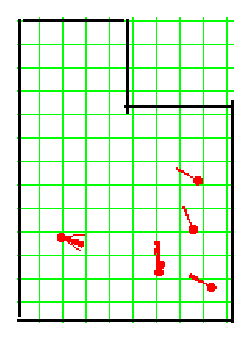
\includegraphics[scale=1]{figuras/cen3_ex1/4.eps}
  \caption[Terceiro Ciclo de Filtragem]{Terceiro ciclo de filtragem}
  \label{img:cen3_ex1_4}
\end{figure}

\begin{figure}[H]
  \centering
  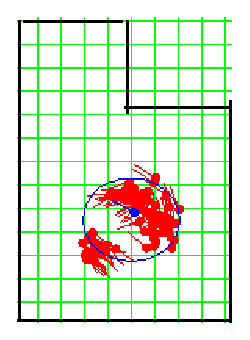
\includegraphics[scale=1]{figuras/cen3_ex1/5.eps}
  \caption[Quarto Ciclo de Filtragem]{Quarto ciclo de filtragem}
  \label{img:cen3_ex1_5}
\end{figure}

\begin{figure}[H]
  \centering
  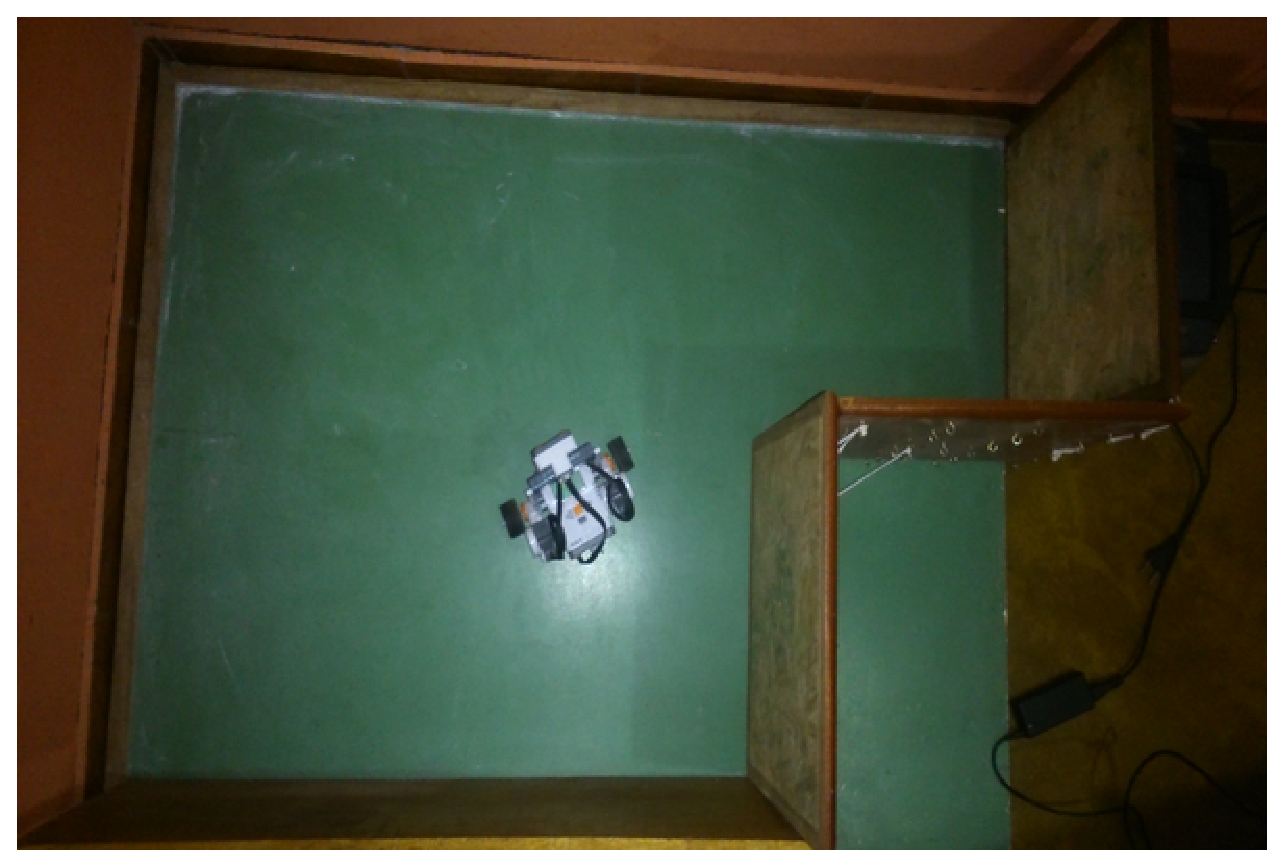
\includegraphics[scale=1]{figuras/cen3_ex1/real.eps}
  \caption[Posição Real do Robô]{Posição Real do Robô.}
  \label{img:cen3_ex1_real}
\end{figure}


\subsection{Exemplo 2}

Exemplo utilizando velocidade de deslocamento em 5 unidades de diâmetro por segundo:

\begin{figure}[H]
  \centering
  \includegraphics[scale=1]{figuras/cen3_ex2/1.eps}
  \caption[Partículas Iniciais]{Partículas iniciais}
  \label{img:cen3_ex2_1}
\end{figure}

\begin{figure}[H]
  \centering
  \includegraphics[scale=1]{figuras/cen3_ex2/2.eps}
  \caption[Primeiro Ciclo de Filtragem]{Primeiro ciclo de filtragem}
  \label{img:cen3_ex2_2}
\end{figure}

\begin{figure}[H]
  \centering
  \includegraphics[scale=1]{figuras/cen3_ex2/3.eps}
  \caption[Segundo Ciclo de Filtragem]{Segundo ciclo de filtragem}
  \label{img:cen3_ex2_3}
\end{figure}

\begin{figure}[H]
  \centering
  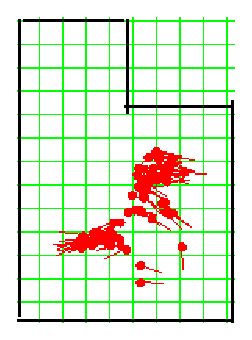
\includegraphics[scale=1]{figuras/cen3_ex2/4.eps}
  \caption[Terceiro Ciclo de Filtragem]{Terceiro ciclo de filtragem}
  \label{img:cen3_ex2_4}
\end{figure}

\begin{figure}[H]
  \centering
  \includegraphics[scale=1]{figuras/cen3_ex2/5.eps}
  \caption[Quarto Ciclo de Filtragem]{Quarto ciclo de filtragem}
  \label{img:cen3_ex2_5}
\end{figure}

\begin{figure}[H]
  \centering
  \includegraphics[scale=1]{figuras/cen3_ex2/6.eps}
  \caption[Quinto Ciclo de Filtragem]{Quinto ciclo de filtragem}
  \label{img:cen3_ex2_6}
\end{figure}

\begin{figure}[H]
  \centering
  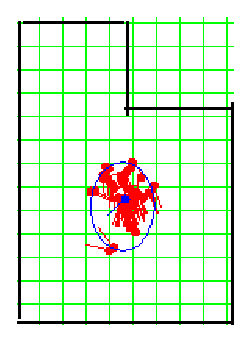
\includegraphics[scale=1]{figuras/cen3_ex2/7.eps}
  \caption[Sexto Ciclo de Filtragem]{Sexto ciclo de filtragem}
  \label{img:cen3_ex2_7}
\end{figure}

\begin{figure}[H]
  \centering
  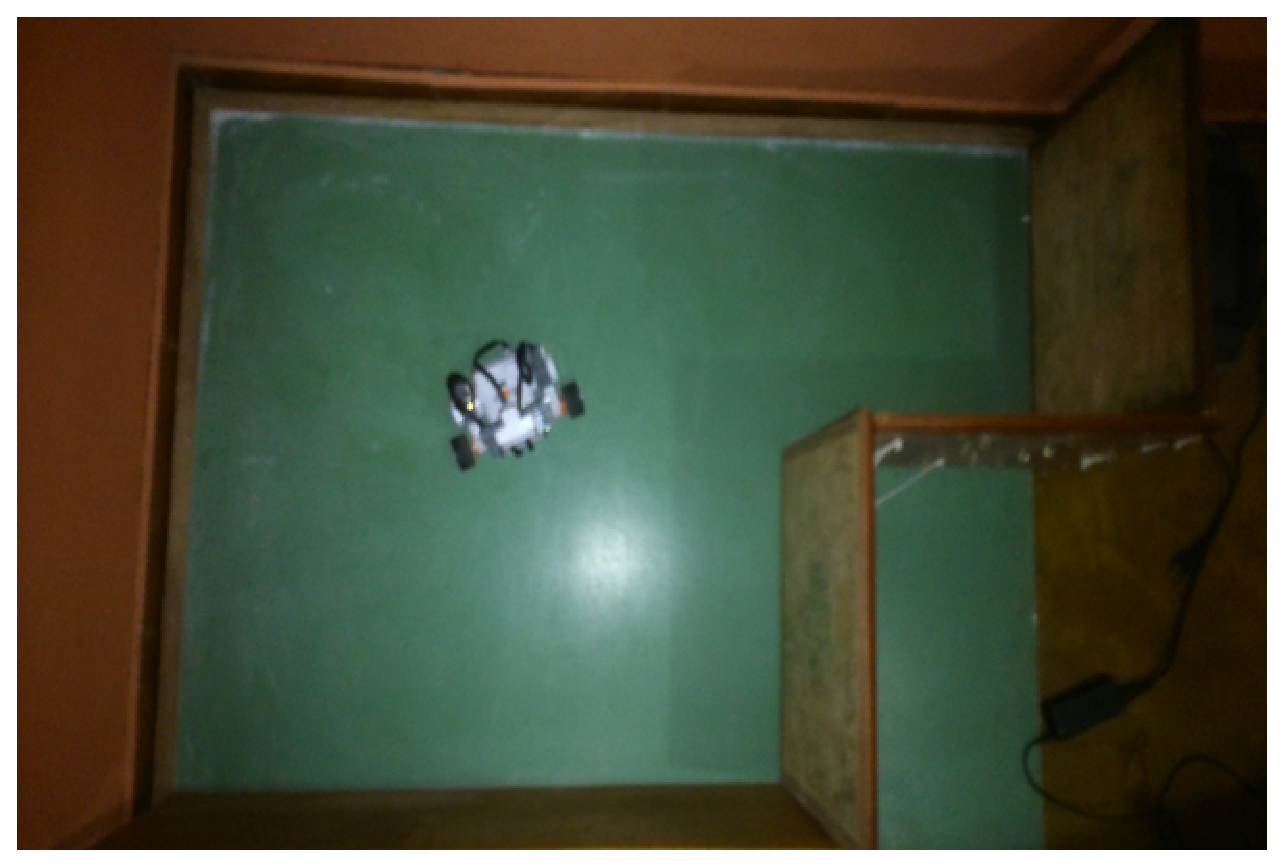
\includegraphics[scale=1]{figuras/cen3_ex2/real.eps}
  \caption[Posição Real do Robô]{Posição Real do Robô.}
  \label{img:cen3_ex2_real}
\end{figure}


\subsection{Exemplo 3}

Exemplo utilizando velocidade de deslocamento em 10 unidades de diâmetro por segundo:

\begin{figure}[H]
  \centering
  \includegraphics[scale=1]{figuras/cen3_ex3/1.eps}
  \caption[Partículas Iniciais]{Partículas iniciais}
  \label{img:cen3_ex3_1}
\end{figure}

\begin{figure}[H]
  \centering
  \includegraphics[scale=1]{figuras/cen3_ex3/2.eps}
  \caption[Primeiro Ciclo de Filtragem]{Primeiro ciclo de filtragem}
  \label{img:cen3_ex3_2}
\end{figure}

\begin{figure}[H]
  \centering
  \includegraphics[scale=1]{figuras/cen3_ex3/3.eps}
  \caption[Segundo Ciclo de Filtragem]{Segundo ciclo de filtragem}
  \label{img:cen3_ex3_3}
\end{figure}

\begin{figure}[H]
  \centering
  \includegraphics[scale=1]{figuras/cen3_ex3/4.eps}
  \caption[Terceiro Ciclo de Filtragem]{Terceiro ciclo de filtragem}
  \label{img:cen3_ex3_4}
\end{figure}

\begin{figure}[H]
  \centering
  \includegraphics[scale=1]{figuras/cen3_ex3/5.eps}
  \caption[Quarto Ciclo de Filtragem]{Quarto ciclo de filtragem}
  \label{img:cen3_ex3_5}
\end{figure}

\begin{figure}[H]
  \centering
  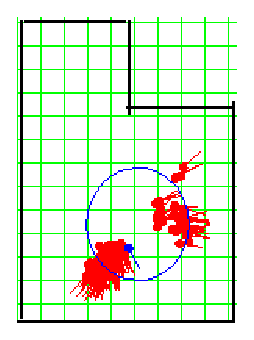
\includegraphics[scale=1]{figuras/cen3_ex3/6.eps}
  \caption[Quinto Ciclo de Filtragem]{Quinto ciclo de filtragem}
  \label{img:cen3_ex3_6}
\end{figure}

\begin{figure}[H]
  \centering
  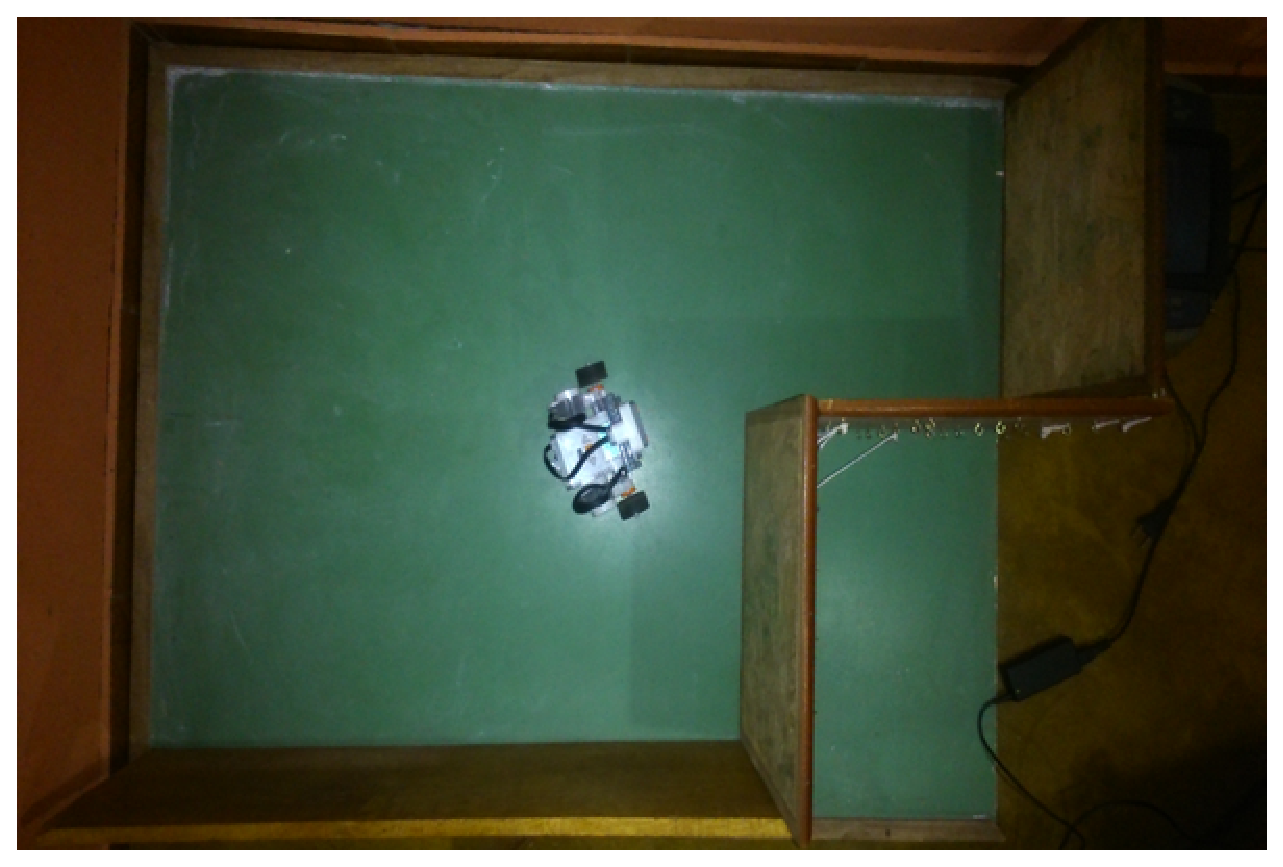
\includegraphics[scale=1]{figuras/cen3_ex3/real.eps}
  \caption[Posição Real do Robô]{Posição Real do Robô.}
  \label{img:cen3_ex3_real}
\end{figure}

\subsection{Exemplo 4}

Exemplo utilizando velocidade de deslocamento em 15 unidades de diâmetro por segundo:

\begin{figure}[H]
  \centering
  \includegraphics[scale=1]{figuras/cen3_ex4/1.eps}
  \caption[Partículas Iniciais]{Partículas iniciais}
  \label{img:cen3_ex4_1}
\end{figure}

\begin{figure}[H]
  \centering
  \includegraphics[scale=1]{figuras/cen3_ex4/2.eps}
  \caption[Primeiro Ciclo de Filtragem]{Primeiro ciclo de filtragem}
  \label{img:cen3_ex4_2}
\end{figure}

\begin{figure}[H]
  \centering
  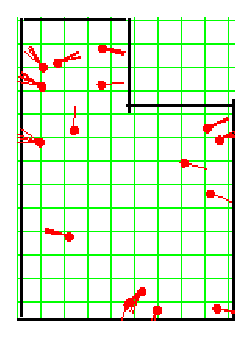
\includegraphics[scale=1]{figuras/cen3_ex4/3.eps}
  \caption[Segundo Ciclo de Filtragem]{Segundo ciclo de filtragem}
  \label{img:cen3_ex4_3}
\end{figure}

\begin{figure}[H]
  \centering
  \includegraphics[scale=1]{figuras/cen3_ex4/4.eps}
  \caption[Terceiro Ciclo de Filtragem]{Terceiro ciclo de filtragem}
  \label{img:cen3_ex4_4}
\end{figure}

\begin{figure}[H]
  \centering
  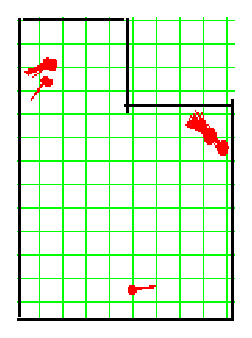
\includegraphics[scale=1]{figuras/cen3_ex4/5.eps}
  \caption[Quarto Ciclo de Filtragem]{Quarto ciclo de filtragem}
  \label{img:cen3_ex4_5}
\end{figure}

\begin{figure}[H]
  \centering
  \includegraphics[scale=1]{figuras/cen3_ex4/6.eps}
  \caption[Quinto Ciclo de Filtragem]{Quinto ciclo de filtragem}
  \label{img:cen3_ex4_6}
\end{figure}

\begin{figure}[H]
  \centering
  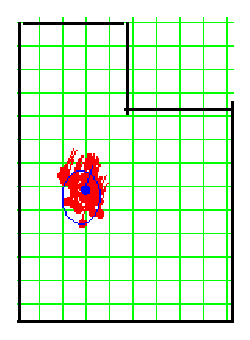
\includegraphics[scale=1]{figuras/cen3_ex4/7.eps}
  \caption[Sexto Ciclo de Filtragem]{Sexto ciclo de filtragem}
  \label{img:cen3_ex4_7}
\end{figure}

\begin{figure}[H]
  \centering
  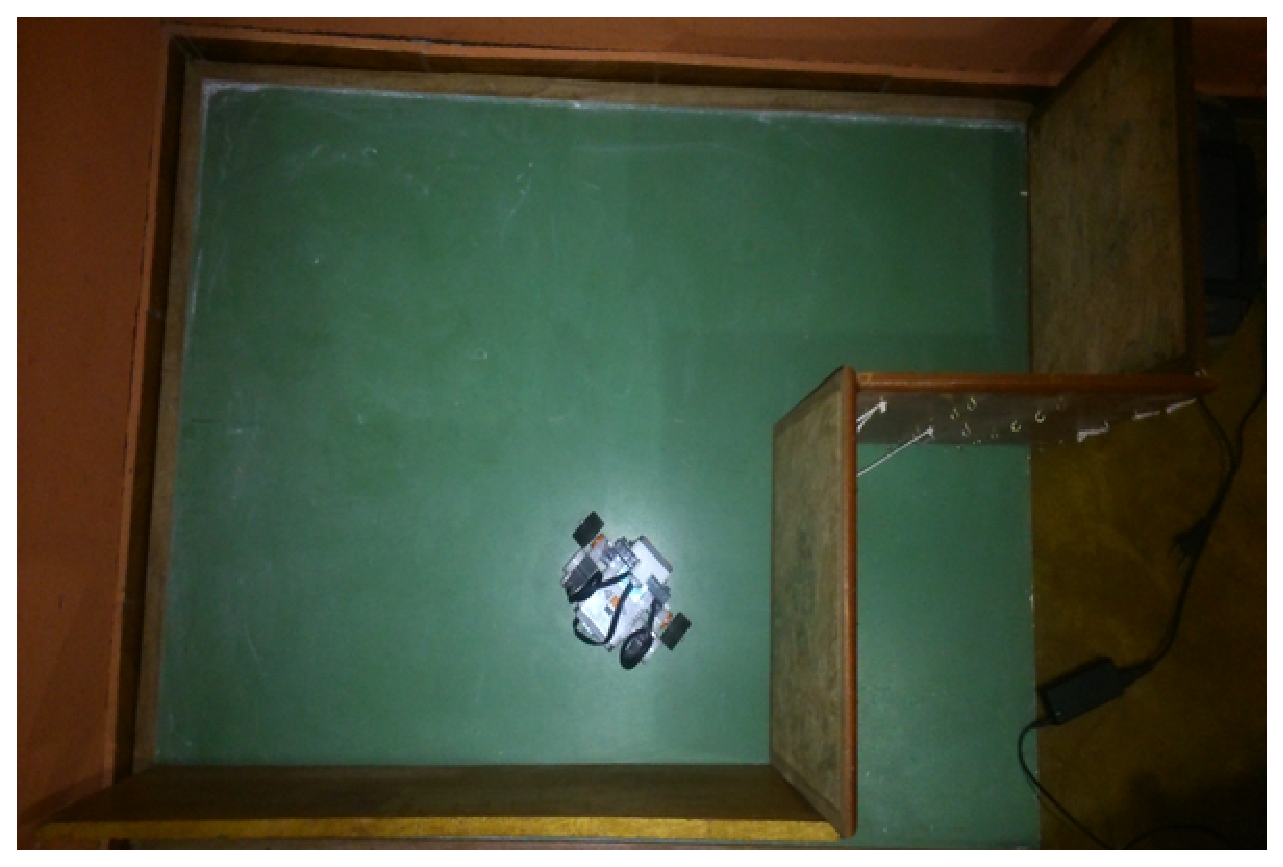
\includegraphics[scale=1]{figuras/cen3_ex4/real.eps}
  \caption[Posição Real do Robô]{Posição Real do Robô.}
  \label{img:cen3_ex4_real}
\end{figure}


\subsection{Exemplo 5}

Exemplo utilizando velocidade de deslocamento em 30 unidades de diâmetro por segundo:

\begin{figure}[H]
  \centering
  \includegraphics[scale=1]{figuras/cen3_ex5/1.eps}
  \caption[Partículas Iniciais]{Partículas iniciais}
  \label{img:cen3_ex5_1}
\end{figure}

\begin{figure}[H]
  \centering
  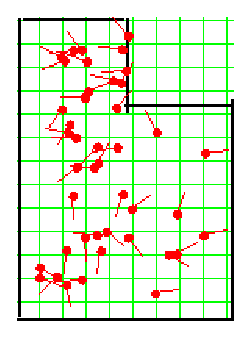
\includegraphics[scale=1]{figuras/cen3_ex5/2.eps}
  \caption[Primeiro Ciclo de Filtragem]{Primeiro ciclo de filtragem}
  \label{img:cen3_ex5_2}
\end{figure}

\begin{figure}[H]
  \centering
  \includegraphics[scale=1]{figuras/cen3_ex5/3.eps}
  \caption[Segundo Ciclo de Filtragem]{Segundo ciclo de filtragem}
  \label{img:cen3_ex5_3}
\end{figure}

\begin{figure}[H]
  \centering
  \includegraphics[scale=1]{figuras/cen3_ex5/4.eps}
  \caption[Terceiro Ciclo de Filtragem]{Terceiro ciclo de filtragem}
  \label{img:cen3_ex5_4}
\end{figure}

\begin{figure}[H]
  \centering
  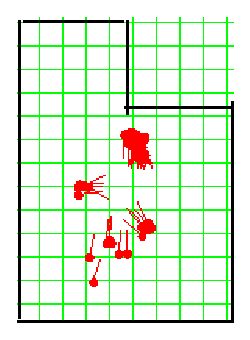
\includegraphics[scale=1]{figuras/cen3_ex5/5.eps}
  \caption[Quarto Ciclo de Filtragem]{Quarto ciclo de filtragem}
  \label{img:cen3_ex5_5}
\end{figure}

\begin{figure}[H]
  \centering
  \includegraphics[scale=1]{figuras/cen3_ex5/6.eps}
  \caption[Quinto Ciclo de Filtragem]{Quinto ciclo de filtragem}
  \label{img:cen3_ex5_6}
\end{figure}

\begin{figure}[H]
  \centering
  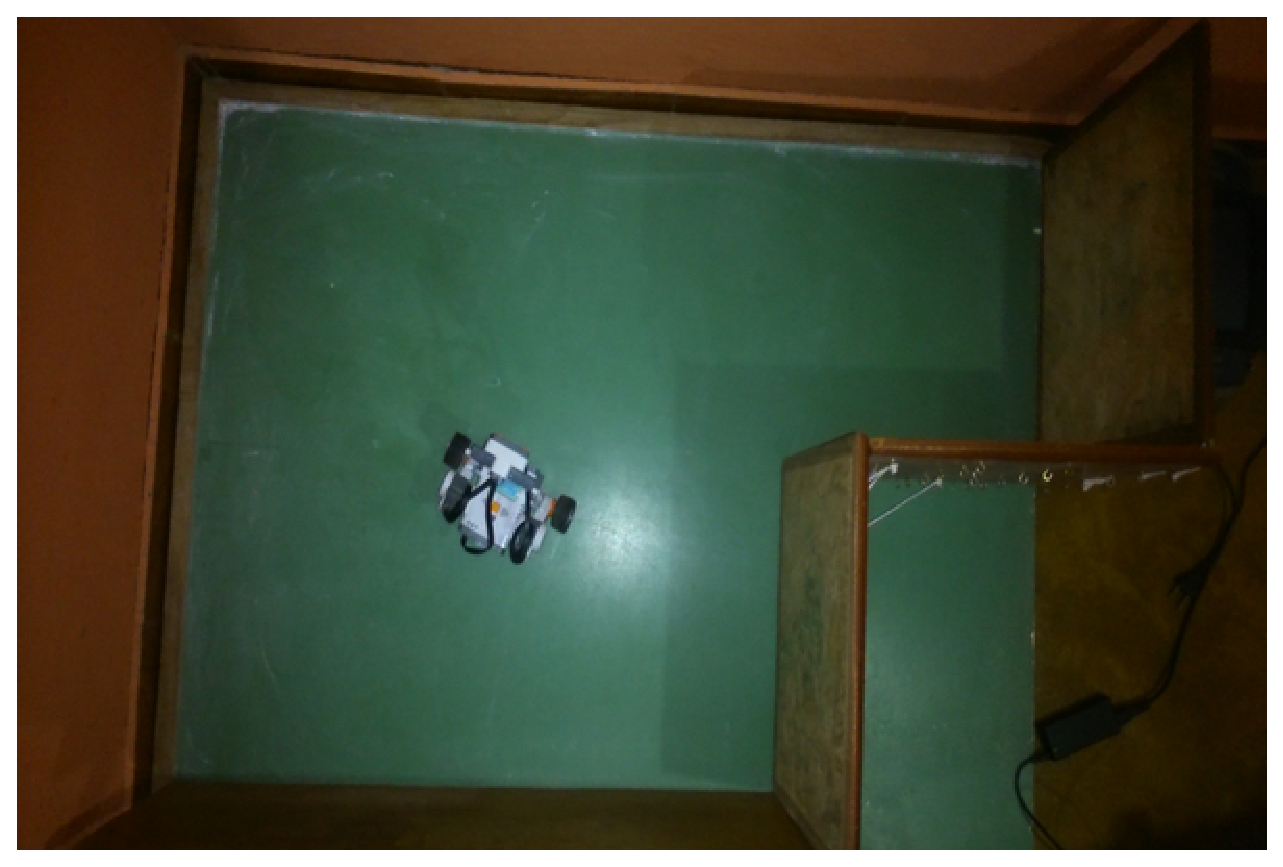
\includegraphics[scale=1]{figuras/cen3_ex5/real.eps}
  \caption[Posição Real do Robô]{Posição Real do Robô.}
  \label{img:cen3_ex5_real}
\end{figure}
